\documentclass[12pt]{exam}

\usepackage{setspace}
\usepackage{listings}
\usepackage{subcaption}
\usepackage{float}
\usepackage{hyperref}
\usepackage{graphicx,wrapfig}
\usepackage{multirow}
\usepackage{amsmath}
\usepackage{bidihl}
\usepackage{tikz-uml}
%\usepackage{multicol}

\usepackage[margin=20mm]{geometry}
\usepackage{xepersian}
\settextfont{B Nazanin}

\newcommand{\class}{الگوها در مهندسی نرم افزار}

\hypersetup{
    colorlinks=true,
    linkcolor=blue,
    filecolor=magenta,      
    urlcolor=cyan,
    pdftitle={Overleaf Example},
    pdfpagemode=FullScreen,
    }
    
\singlespacing
\parindent 0ex

\lstset{
keywordstyle=\textbf,
identifierstyle=, 
stringstyle=\ttfamily,
commentstyle=\color{LimeGreen}, 
stringstyle=\ttfamily,
numberstyle=\footnotesize,
showstringspaces=false} 
\begin{document}


% -------------------------------------------------------
%  Thesis Information
% -------------------------------------------------------

\newcommand{\ThesisTitle}
{الگوها در سیستم های نهفته بی درنگ}
\newcommand{\ThesisAuthor}
{علی محسنی نژاد}
\newcommand{\ThesisSupervisor}
{دکتر رامان رامسین}
\newcommand{\ThesisDate}
{مرداد ۱۴۰۳}
\newcommand{\ThesisDepartment}
{دانشکده مهندسی کامپیوتر}
\newcommand{\ThesisUniversity}
{دانشگاه صنعتی شریف}

% -------------------------------------------------------
%  English Information
% -------------------------------------------------------

%\newcommand{\EnglishThesisTitle}{A Standard Template for Course Exercise}


\pagestyle{empty}

\begin{center}


\includegraphics[scale=0.2]{images/logo.png}

\vspace{0.5cm}
\ThesisUniversity \\[-0.3em]
\vspace{0.5cm}
\ThesisDepartment\\

\begin{large}
\vspace{0.5cm}


%\ThesisMajor

\end{large}

\vspace{1.5cm}

{عنوان:}\\[1.2em]
{\LARGE\textbf{\ThesisTitle}}\\ 
\vspace{1cm}
%\begin{latin}
%{\Large\textbf\EnglishThesisTitle}
%\end{latin}

\vspace{2cm}

{نویسنده}\\[.5em]
{\large\textbf{\ThesisAuthor}}

\vspace{1.5cm}

{استاد}\\[.5em]
{\large\textbf{\ThesisSupervisor}}

\vspace{1cm}



\vspace{2cm}

\ThesisDate

\end{center}

\newpage

\tableofcontents
% These commands set up the running header on the top of the exam pages
\pagestyle{head}
\firstpageheader{}{}{}
\runningheader{صفحه \thepage\ از \numpages}{}{\class}
\runningheadrule


\setlength\parindent{24pt}
\section{مقدمه}

\begin{RTL}
این گزارش به طور مفصل به توضیح الگوهای معرفی‌شده در مقالات و کتب مختلف
در حوزه سیستم‌های نهفته و بی‌درنگ می‌پردازد.
برای درک عمیق‌تر این الگوها، باید ابتدا مشخص شود که منظور
از سیستم‌های نهفته بی‌درنگ چیست.
سیستم‌های نهفته در بخش‌های زیادی از زندگی روزمره وجود دارند؛
به طور مثال سیستم‌های رادیویی، سیستم‌های ناوبری، سیستم‌های تصویربرداری.
به طور کلی یک سیستم نهفته را می‌توان اینگونه تعریف کرد،:
«یک سیستم کامپیوتری که به طور مشخص برای انجام یک کار در دنیای واقعی
تخصیص داده‌شده و هدف آن ایجاد یک محیط کامپیوتری
با کاربری عام نیست» \cite{ref1}.
یک دسته مهم از سیستم‌های نهفته، سیستم‌های بی‌درنگ هستند.
«سیستم‌های بی‌درنگ، سیستم‌هایی
هستند که در آن‌ها قیدهای زمانی مشخص باید برآورده شوند
تا سیستم بتواند به درستی کار کند» \cite{ref1}.
\end{RTL}

\begin{RTL}
حال که مفهوم سیستم‌های نهفته بی‌درنگ را دریافتیم، باید تعریفی از الگو در این سیستم‌ها
ارائه دهیم. منابع متنوع تعاریف متفاوتی از الگوها ارائه کرده‌اند و بسیاری از آن‌ها
این تعریف را به الگوهای طراحی محدود می‌کنند \cite{ref1}.
هدف این گزارش تقسیم‌بندی الگوهای نرم‌افزاری به طور کلی نیست و صرفا می‌خواهیم
الگوهای مورد استفاده در سیستم‌های نهفته و بی‌درنگ را بررسی کنیم.
\lr{Zalewski} \cite{ref2} می‌گوید:
«یک الگو یک مدل یا یک قالب نرم‌افزاری است که به فرایند ایجاد نرم‌افزار کمک می‌کند.»
این تعریف در عین سادگی، جامع است؛ به طوری که الگوهای طراحی، معماری و فرایندی
را در خود شامل می‌شود. با این حال این مقاله نیز مانند بسیاری از دیگر مقالات،
تعریف جدیدی از الگوها در سیستم‌های نهفته بی‌درنگ ارائه نکرده‌اند و برای تعریف آن به
تعریف \lr{Gamma} و دیگران \cite{ref3} از الگوهای طراحی ارجاع داده‌اند.
\end{RTL}

\begin{RTL}
\bidihl{
    ساختار گزارش و مطالبی که گفته می‌شود.
}
\end{RTL}


\section{الگوهای طراحی برای دسترسی به سخت‌افزار}
\begin{RTL}
نرم‌افزارهای نهفته بر روی یک بستر سخت‌افزاری مستقر می‌شوند و معمولا بسیاری از قابلیت‌های
آن‌ها ملزم به ارتباط با سخت‌افزار می‌شود. به همین دلیل \lr{Douglass}
\cite{ref1} یک دسته از الگوها را با عنوان الگوهای دسترسی به سخت‌افزار
معرفی می‌کند.
\end{RTL}
\subsection{الگوی \lr{Hardware Proxy}}
\label{HWProxySec}
\begin{RTL}
این الگو با ایجاد یک رابط روی یک جزء سخت‌افزاری، یک دسترسی
مستقل از پیچیدگی‌های اتصال به سخت‌افزار برای کلاینت ایجاد می‌کند.
این الگو با معرفی یک کلاس به نام پروکسی بین سخت‌افزار و کلاینت،
باعث می‌شود که تمامی عملیات وابسته به سخت‌افزار در پروکسی انجام شود
و در صورت تغییر در سخت‌افزار، هیچ تغییری به کلاینت تحمیل نشود.
در این الگو بر روی یک جزء سخت‌افزاری، یک پروکسی قرار گرفته و
کلاینتان متعدد می‌توانند از آن سرویس بگیرند. لازم به ذکر است که ارتباط پروکسی
و سخت‌افزار بر پایه یک «رابط قابل آدرس‌دهی توسط نرم‌افزار» است. 
دیاگرام کلاس این الگو در شکل \ref{HWProxyClassDiag} رسم شده‌است.
\end{RTL}
\begin{figure}[h!]
\centering
\begin{tikzpicture}
\lr{
  \umlclass{HardwareProxy}{
    device\_address
  }{
    initialize()\\
    configure()\\
    disable()\\
    access()\\
    mutate()
  }
  \umlclass[y=-6]{HardwareDevice}{
    \lr{}
  }{}
  \umlclass[x=5]{ProxyClient}{
    \lr{}
  }{}
\umlassoc[mult1=1, mult2=1]{HardwareProxy}{HardwareDevice}
\umluniassoc[mult1=1..*, mult2=1]{ProxyClient}{HardwareProxy}
}
\end{tikzpicture}
\caption{دیاگرام کلاس \lr{Hardware Proxy}}
\label{HWProxyClassDiag}
\end{figure}
\begin{RTL}
همانطور که در شکل \ref{HWProxyClassDiag} دیده می‌شود، کلاس پروکسی توابع
مشخصی را در اختیار کلاینت‌ها قرار می‌دهد\footnote{توابع دیگری نیز در \cite{ref1}
گفته‌شده ولی اینجا تنها توابع \lr{public} کلاس پروکسی را بررسی می‌کنیم.}.
توضیحات مربوط به هر یک از توابع کلاس پروکسی در شکل زیر داده شده‌است:
\begin{itemize}
  \item \lr{initialize}:
  این تابع برای آماده‌سازی اولیه ارتباط با سخت‌افزار استفاده می‌شود و معمولا تنها یک بار
  صدا زده می‌شود.
  \item \lr{configure}:
  این تابع برای ارسال تنظیمات برای سخت‌افزار استفاده می‌شود. معمولا باید در سخت‌افزار
  تنظیماتی قرار داده‌شود که آن را قابل استفاده کند.
  \item \lr{disable}:
  این تابع برای غیرفعال‌کردن سخت‌افزار به صورت امن استفاده می‌شود.
  \item \lr{access}:
  این تابع برای دریافت اطلاعات از طرف سخت‌افزار استفاده می‌شود.
  \item \lr{mutate}:
  این تابع برای فرستادن اطلاعات به سمت سخت‌افزار استفاده می‌شود.
\end{itemize}
\end{RTL}
\subsection{الگوی \lr{Hardware Adapter}}
\label{HWAdapterSec}
\begin{RTL}
این الگو مشابه الگوی \lr{Adapter} که \lr{Gamma} و دیگران
\cite{ref3} معرفی کرده‌اند تعریف شده. استفاده از این الگو این اجازه را
می‌دهد که کلاینتی که انتظار یک رابط خاص با سخت‌افزار را دارد، بتواند با
سخت‌افزارهای مختلف بدون این‌که متوجه تفاوت‌های آن‌ها شود ارتباط بگیرد.
این الگو روی ساختار \nameref{HWProxySec} بنا شده‌است و
دیاگرام کلاس آن در شکل \ref{HWAdapterClassDiag} ترسیم شده‌است.
\end{RTL}
\begin{figure}[h!]
\centering
\begin{tikzpicture}
\lr{
    \umlclass{HardwareProxy}{
    device\_address
    }{
    initialize()\\
    configure()\\
    disable()\\
    access()\\
    mutate()
    }
    \umlclass[y=-6]{HardwareDevice}{
    \lr{}
    }{}
    \umlclass[x=6]{HardwareAdapter}{
    \lr{}
    }{
        clientService1() \\
        clientService2()
    }
    \umlinterface[x=6, y=4]{HardwareInterfaceToClient}{}{
        \umlvirt{clientService1()} \\
        \umlvirt{clientService2()}
    }
    \umlclass[x=13, y=4]{AdapterClient}{
        \lr{}
    }{}
\umlassoc[mult1=1, mult2=1]{HardwareProxy}{HardwareDevice}
\umluniassoc[mult1=1..*, mult2=1]{HardwareAdapter}{HardwareProxy}
\umlimpl[]{HardwareAdapter}{HardwareInterfaceToClient}
\umlassoc[mult1=1, mult2=1]{AdapterClient}{HardwareInterfaceToClient}
}
\end{tikzpicture}
\caption{دیاگرام کلاس \lr{Hardware Adapter}}
\label{HWAdapterClassDiag}
\end{figure}
\begin{RTL}
همانطور که در شکل \ref{HWAdapterClassDiag} دیده می‌شود،
کلاس کلاینت سرویس‌های مورد انتظار خود را از رابط
\lr{HardwareInterfaceToClient} انتظار دارد.
در این ساختار، کلاس آداپتور، سرویس‌های مورد انتظار کلاینت را به سرویس‌های ارائه‌شده
از طرف سخت‌افزار ترجمه می‌کند. این کار اجازه می‌دهد که در صورت تغییر سخت‌افزار
(و متناظرا پروکسی)، تنها با ایجاد پیاده‌سازی جدید برای رابط آداپتور، نیازی به تغییر
در کلاینت نباشد.
\end{RTL}



% \umlassoc[geometry=-|-,
%   arg1=tata,
%   mult1=*,
%   pos1=1.3,
%   arg2=toto,
%   align1=bottom,
%   mult2=1,
%   pos2=1.7,
%   align2=top
% ]{Proxy}{Hardware}
\subsection{الگوهای طراحی برای ماشین‌های حالت}
\begin{RTL}
این دسته از الگوها که توسط \lr{Douglass} در \cite{ref1}
معرفی شده‌است، الگوهایی هستند که براساس ماشین‌های حالت ساخته شده‌اند.
\end{RTL}
\subsubsection{الگوی \lr{Single Event Receptor}}
\label{smSingleEvRecSec}
\begin{RTL}
این الگو یک دریافت‌کننده رویداد را به کلاینت‌ها عرضه می‌کند که می‌تواند رویدادهای
سنکرون و آسنکرون را دریافت کند. در این الگو، ورودی این دریافت‌کنند علاوه بر
نوع رویدادی که رخ‌داده‌است، باید دارای داده‌های مربوط به رویداد نیز باشد. 
\end{RTL}
\subsubsection{الگوی \lr{Multiple Event Receptor}}
\subsubsection{الگوی \lr{State Table}}
\subsubsection{الگوی \lr{State}}
\label{smStateSec}
\begin{RTL}
این الگو \cite{ref1} با واسپاری حالت سیستم به یک شیء
مجزا، وظیفه مدیریت حالت را به آن می‌دهد. در این الگو، تمامی رویدادهای دریافتی
به این شیء پاس داده می‌شوند و او با توجه به این که حالت بعدی را می‌شناسد،
خود را با شیء مربوط به حالت جدید جایگزین می‌کند.
در این ساختار، با اضافه‌شدن هر حالت جدید، باید یک کلاس جدید تعریف شود.
این الگو نسبت به \nameref{smStateTableSec} حافظه بیشتری اشغال
می‌کند اما با توزیع وظیفه مدیریت حالت بین کلاس‌های مختلف، پیاده‌سازی
ساده‌تری دارد. یکی دیگر از مزیت‌های استفاده از این الگو، این است که
این کلاس‌های حالت را می‌توان بین کلاینت‌های مختلف به اشتراک گذاشت.
\end{RTL}
\subsubsection{الگوی \lr{Decomposed And State}}
\label{smDecomAndStateSec}
\begin{RTL}
این الگو \cite{ref1}، با استفاده از
\nameref{smStateSec} می‌خواهد \lr{AND-State}ها را
با ایجاد همکاری میان اشیاء مختلف که هر کدام یک \lr{AND-State}
را مدیریت می‌کند، مدیریت کند.
شیء اصلی، ماشین حالت کلی را نظارت می‌کند، در حالی که اشیاء دیگر
\lr{AND-State}های تکی را مدیریت می‌کند. این الگو به پیاده‌سازی
ماشین‌هایحالت با منطق‌های مستقل می‌پردازد و
طراحی \lr{AND-State}ها را حفظ می‌کند.
این الگو مدیریت حالت را از طریق واگذاری مسئولیت‌ها ساده می‌کند،
اما نیاز به مدیریت دقیق لیست‌ها و اشاره‌گرها دارد تا
از بروز خطاهای نامشخص جلوگیری شود.
\end{RTL}
\section{الگوهای طراحی برای ماشین‌های حالت}
\begin{RTL}

\end{RTL}
\subsection{الگوی \lr{Single Event Receptor}}
\subsection{الگوی \lr{Multiple Event Receptor}}
\subsection{الگوی \lr{State Table}}
\subsection{الگوی \lr{State}}
\subsection{\lr{And States}}
\subsection{الگوی \lr{Decomposed And State}}
\subsection{الگوهای معماری زیربخش‌ها و اجزا}
\begin{RTL}

\end{RTL}
\subsubsection{الگوی \lr{Layered}}
\label{archLayerSec}
\begin{RTL}
الگوی لایه‌ای \cite{ref4} دامنه‌های سیستم را بر اساس سطوح انتزاعی
مختلف به صورت سلسله‌مراتبی
سازمان‌دهی می‌کند. مفاهیم انتزاعی‌تر در یک دامنه با استفاده
از مفاهیم ملموس‌تر در دامنه‌های دیگر پیاده‌سازی می‌شوند.
این ساختار به متخصصان اجازه می‌دهد تا به طور موثر در زمینه تخصصی
خود کار کنند بدون اینکه نیاز به درک تمامی جزئیات زیرین
داشته باشند. به همین ترتیب، در توسعه نرم‌افزار،
دامنه‌های انتزاعی با استفاده از دامنه‌های ملموس‌تر پیاده‌سازی
می‌شوند که این امر موجب سازمان‌دهی و قابلیت تطبیق‌پذیری بیشتر بین
پلتفرم‌های مختلف می‌شود.
\end{RTL}
\begin{figure}[h!]
\centering
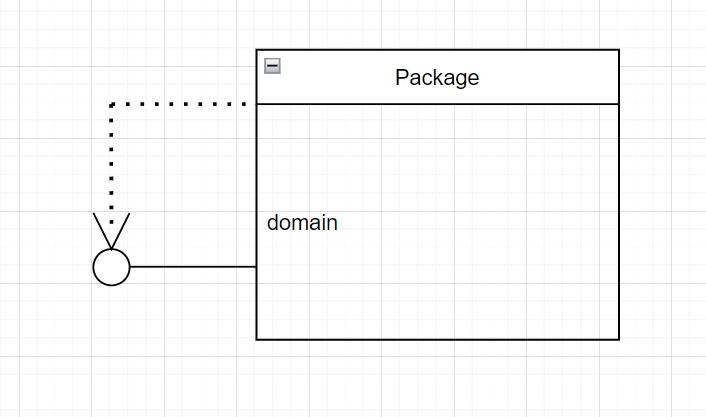
\includegraphics[scale=0.5]{images/first/layer.png}
\caption{ساختار الگوی \lr{Layered}}
\end{figure}
\subsubsection{الگوی \lr{Five Layer}}
\label{arch5LayerSec}
\begin{RTL}
الگوی معماری پنج‌لایه یک تطبیق خاص از \nameref{archLayerSec} است
که برای ساختاردهی بسیاری از سیستم‌های نهفته و بی‌درنگ
مفید است. این الگو معماری منطقی را به پنج لایه
تقسیم می‌کند که این امر به توسعه‌دهندگان کمک می‌کند
تا به راحتی ساختار سیستم‌های جدید را درک کنند.
این الگو از قابلیت انتقال بین پلتفرم‌های مختلف پشتیبانی
می‌کند و یک پلتفرم انتزاعی فراهم می‌کند که تطبیق برنامه‌ها
را آسان‌تر می‌سازد. در حالی که این الگو بسیاری از
مزایای \nameref{archLayerSec} را دارد، از جمله کارایی بالا به دلیل تعداد
کم لایه‌ها، ممکن است برای تجزیه کافی سیستم‌های پیچیده مناسب نباشد.
\end{RTL}
\subsubsection{الگوی \lr{Microkernel}}
\subsection{الگوی \lr{Channel}}
\subsubsection{الگوی \lr{Recursive Containment}}
\label{archRecContainSec}
\begin{RTL}
الگوی تجزیه و تحلیل بازگشتی برای مدیریت سیستم‌های بسیار پیچیده
با نیازمندی‌های فراوان مؤثر است. این الگو شامل شکستن سیستم به
اجزای مرتبط در سطوح مختلف جزئیات است، مانند استفاده از میکروسکوپ
با سطوح مختلف بزرگ‌نمایی. در هر سطح، اشیاء واسط‌هایی
برای همتایان خود فراهم می‌کنند و وظایف را به اجزای کوچک‌تر داخلی
تفویض می‌کنند، این تجزیه و تحلیل به صورت بازگشتی ادامه می‌یابد
تا هر بخش دارای مسئولیت ساده و متمرکز شود. این رویکرد امکان تجزیه
و تحلیل مقیاس‌پذیر را فراهم می‌کند و تأیید موارد استفاده بزرگ انتزاعی
را در هر مرحله ممکن می‌سازد و سطوح مختلفی از جزئیات رفتار سیستم را ارائه می‌دهد.
\end{RTL}
\subsubsection{الگوی \lr{Hierarchical Control}}
\label{archHierContSec}
\begin{RTL}
الگوی کنترل سلسله‌مراتبی \cite{ref4} یک
نسخه تخصصی از \nameref{archRecContainSec}
است که الگوریتم‌های پیچیده کنترلی را بین اجزای مختلف توزیع می‌کند.
این الگو از دو نوع واسط استفاده می‌کند:
واسط‌های کنترلی که نحوه دستیابی به رفتارها را نظارت و کنترل می‌کنند
و واسط‌های عملکردی که خدمات کنترل‌شده توسط واسط‌های دیگر را فراهم می‌کنند.
واسط‌های کنترلی کیفیت خدمات، مانند دقت و صحت، را تعیین می‌کنند
و سیاست‌های اجرایی را تنظیم می‌کنند. واسط‌های عملکردی رفتار مطلوب
را با استفاده از کیفیت خدمات و سیاست‌های تنظیم شده توسط واسط
کنترلی اجرا می‌کنند. این الگو با استفاده از نمودارهای حالت برای
هماهنگی اجزای زیرمجموعه و تجمیع اجزای جزء به کنترل‌کننده
از طریق ترکیب، ساختار سلسله‌مراتبی قابل تنظیم و مقیاس‌پذیری را
فراهم می‌کند. در این الگو، کنترل‌کننده وظیفه هماهنگی درخواست‌های
خدمات به عناصر جزء را دارد و اغلب از نمودارهای حالت برای نشان
دادن حالت‌های تنظیمات اجزای زیرمجموعه استفاده می‌کند. این روش
به ویژه زمانی مفید است که حالت‌های مختلف اجزای زیرمجموعه مستقل
نباشند و با استفاده از نمودارهای حالت و انطباق حالت‌ها، سازگاری میان اجزا حفظ شود.
\end{RTL}
\begin{figure}[h!]
\centering
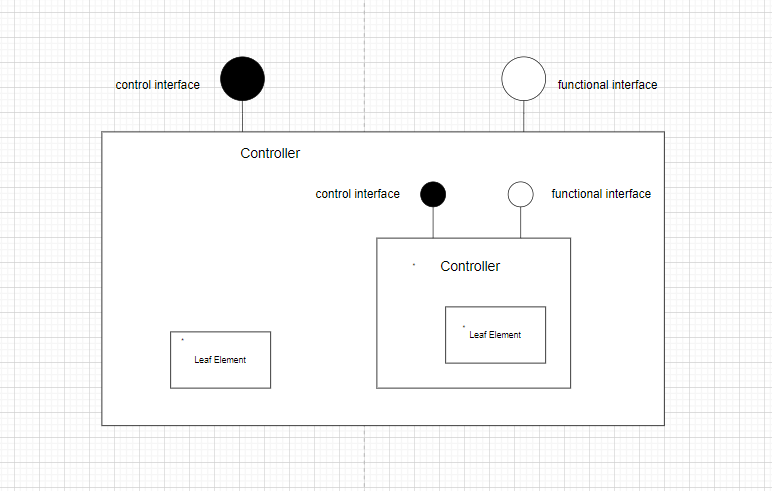
\includegraphics[scale=0.5]{images/first/hierarchical.png}
\caption{ساختار الگوی \lr{Hierarchical Control}}
\end{figure}
\subsubsection{الگوی \lr{Virtual Machine}}
\label{archVirtMachineSec}
\begin{RTL}
الگوی ماشین مجازی \cite{ref4} اولویت را
به قابلیت انتقال برنامه‌ها می‌دهد تا به کارایی
در زمان اجرا، و برای برنامه‌هایی که نیاز به اجرای روی پلتفرم‌های مختلف
دارند اما عملکرد حداکثری ضروری نیست، مناسب است.
برنامه‌ها برای یک ماشین انتزاعی نوشته می‌شوند و یک ماشین مجازی
نرم‌افزاری این دستورات را بر روی سخت‌افزار واقعی تفسیر می‌کند.
این الگو انتقال برنامه‌ها به محیط‌های جدید را ساده می‌کند،
زیرا فقط نیاز است ماشین مجازی برای پلتفرم هدف تطبیق داده شود.
اگرچه برنامه‌ها ممکن است کندتر از برنامه‌های کامپایل شده بومی اجرا
شوند، اما مزایای آن شامل ساده‌سازی انتقال و اندازه کوچکتر برنامه‌ها به
دلیل اشتراک کتابخانه‌ها در داخل ماشین مجازی است. با این حال، ماشین‌های
مجازی می‌توانند منابع زیادی مصرف کنند و ممکن است برای دستگاه‌های با
محدودیت حافظه مناسب نباشند. در چنین شرایطی ممکن است الگویی مانند
\nameref{archMicrokernelSec}
مناسب‌تر باشد.
\end{RTL}
\begin{figure}[h!]
\centering
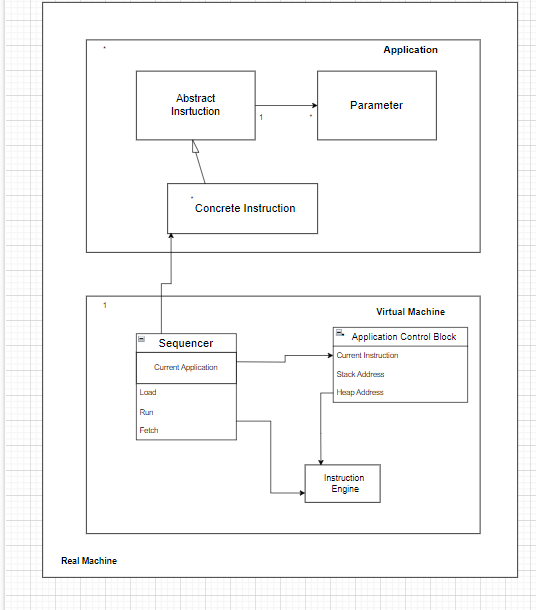
\includegraphics[scale=0.8]{images/first/virtual_machine.png}
\caption{ساختار الگوی \lr{Virtual Machine}}
\end{figure}
\subsubsection{معماری \lr{Component-Based}}
\label{archCompBasedSec}
\begin{RTL}
در \lr{UML}،
یک \lr{Component} یک اثر زمان اجرا و یک واحد قابل
جایگزینی اساسی در نرم‌افزار است
که مشابه یک شیء بزرگ‌مقیاس شامل اشیاء کوچکتری است که واسط آن را
پیاده‌سازی می‌کنند. \lr{Component}ها دارای کپسوله‌سازی قوی و
واسط‌های مستقل از زبان برنامه‌نویسی و کاملاً تعریف شده هستند.
سیستم‌های مبتنی بر \lr{Component}
که از این اشیاء بزرگ‌مقیاس به عنوان واحدهای معماری استفاده می‌کنند، از نگهداری
آسان، جداسازی عیوب، استقلال از زبان منبع، سادگی توسعه و قابلیت استفاده مجدد
بهره‌مند می‌شوند. \lr{Component}ها معمولاً اشیاء کوچکتری را
برای هدف رفتاری مشترک زمان اجرا جمع می‌کنند.
آنها دارای واسط‌های مبهم هستند، به این معنا که جزئیات
داخلی آنها از کلاینت مخفی است که این امر جایگزینی را تضمین می‌کند
اما ممکن است منجر به ناکارآمدی شود. الگوی معماری مبتنی بر مؤلفه معماری
سیستم را قوی و قابل استفاده مجدد فراهم می‌کند اما ممکن است به دلیل
استفاده از کل \lr{Component}ها حتی اگر فقط بخشی از عملکرد آنها
استفاده شود، منابع اضافی مصرف کند.
\end{RTL}
\subsubsection{الگوی \lr{ROOM}}
\section{مراجع}
\renewcommand{\section}[2]{}%
\begin{thebibliography}{1}
    
\bibitem{ref1}
\lr{Douglass, Bruce Powel. Design patterns for embedded systems in C: an embedded software engineering toolkit. Elsevier, 2010.}
\bibitem{ref2}
\lr{Zalewski, Janusz. "Real-time software architectures and design patterns: Fundamental concepts and their consequences." Annual Reviews in Control 25 (2001): 133-146.}
\bibitem{ref3}
\lr{Gamma, Erich, et al. "Design patterns: Abstraction and reuse of object-oriented design." ECOOP’93—Object-Oriented Programming: 7th European Conference Kaiserslautern, Germany, July 26–30, 1993 Proceedings 7. Springer Berlin Heidelberg, 1993.}
\bibitem{ref4}
\lr{Douglass, Bruce Powel. Real-time design patterns: robust scalable architecture for real-time systems. Addison-Wesley Professional, 2003.}
\end{thebibliography}
% \include{part2.tex}




\end{document}